%%%%%%%%%%%%%%%%%%%%%%%%%%%%%%%%%%%%%%%%%%%%%%%%%%%%%%%%%%%%%%%%%%%%%%%%
%%        Annotated example of a homework submission in LaTeX         %%
%%               (note: LaTeX comments begin with a %)                %%
%%%%%%%%%%%%%%%%%%%%%%%%%%%%%%%%%%%%%%%%%%%%%%%%%%%%%%%%%%%%%%%%%%%%%%%%

%% Build this document with
%%
%%   pdflatex annotated_homework_example.tex
%%
%% or
%%
%%   latex annotated_homework_example.tex
%%   dvips annotated_homework_example.dvi
%%   ps2pdf annotated_homework_example.ps
%%
%% The result will be annotated_homework_example.pdf.
%%
%% IMPORTANT NOTE: Because this sample uses cross references, you must
%% build it *TWICE*. LaTeX finds all of the cross reference TARGETS first
%% and then, on the second run, plugs them all in to the appropriate
%% places.
%%
%% (note: any good LaTeX-friendly text editor will have these build
%%  lines built into it)

%%%%%%%%%%%%%%%%%%%%%%%%%%%%%%% PREAMBLE %%%%%%%%%%%%%%%%%%%%%%%%%%%%%%%

%% Every LaTeX document starts with a \documentclass line. The
%% document class sets up the most prominent features of the document
%% style (e.g., page styles, font, etc.).
%%
%% Standard document classes include article, book, and report.
%%
%%   *) The article document class is the most commonly used for short
%%      documents. It provides sectioning commands and flexible titling
%%      options.
%%
%%   *) The report document class gives you chapters and puts the title
%%      information centered on a separate unnumbered page.
%%
%%   *) The book document class gives you the ability to make parts and
%%      chapters and is usually used in two-sided printing mode (e.g.,
%%      page numbering alternates from being on the top left to top
%%      right of the page rather than in the bottom center).
%%
%% More advanced document classes include memoir, which is a drop-in
%% replacement for the standard classes that has many other features as
%% well. It folds in a rich feature set from some of the most popular
%% packages (packages are explained below).
%%
%% Optional arguments to LaTeX macros come in square brackets. In this
%% case, [10pt] tells the article class that we want 10 point font.
\documentclass[10pt]{article}

%% The default margins for article may seem large to you. They are
%% designed to look pleasant on a page. To use 1 inch margins instead,
%% call the geometry package with this line:
\usepackage[margin=1in]{geometry}

%% The enumitem package provides nicer list support to LaTeX.
\usepackage[shortlabels]{enumitem}

%% This setcounter line makes it so that \section commands do not have
%% numbers printed in front of them. Delete this line ENTIRELY *OR*
%% change the 0 to 1 or higher to make it so that \section commands
%% automatically get numbered.
%%
%% If you do increase the 0 to a positive integer or remove this line
%% entirely, later you can use \section* to get a single unnumbered
%% section.
\setcounter{secnumdepth}{0}

% The graphicx package lets us include images with \includegraphics
\usepackage{graphicx}
\usepackage{epstopdf}
% The caption package lets us customize captions when we want to make
% formal figures and tables
\usepackage{caption}


%% Here, we use the fancyhdr and lastpage packages to customize the
%% header and footer of each page
\usepackage{fancyhdr, lastpage}
\usepackage{amsmath, amsthm, amssymb}
\pagestyle{fancy}
\fancyhf{}
%
%% Put your name and homework identification here
\lhead{John St. John}
\chead{EE~253~--- \today}
\rhead{Homework 1}
%
\cfoot{Page \thepage{} of \protect\pageref*{LastPage}}

%% These next two lines are only used if you are going to cross
%% reference equations in your submissions. They can probably be removed
%% for 481 submissions.
\usepackage{varioref}
\labelformat{equation}{(#1)}

% The hyperref package automatically links cross references to their
% targets and does LOTS more. In our case, we include it so that we can
% use \autoref. \autoref lets us do \autoref{eq:one} rather than
% Equation~\ref{eq:one}.
%
% We use the colorlinks option here, which colors hyperlinks rather
% than putting boxes around them. We then use the linkcolor option to
% make them blue rather than the default red. We could have used
% [pdfborder={0 0 0}] instead, which would leave the links uncolored,
% but it would remove the boxes.
%
% \usepackage{hyperref} must almost always be LAST \usepackage in
% preamble. Otherwise, you may get strange compilation errors!
\usepackage[colorlinks,linkcolor=blue]{hyperref}

%%%%%%%%%%%%%%%%%%%%%%%% MAIN DOCUMENT CONTENT %%%%%%%%%%%%%%%%%%%%%%%%%

% We surround our main content with a ``document'' ``environment.'' This
% marks the end of our LaTeX setup and the start of our document output.
%
% All ``environments'' are identified by \begin{...} and \end{...}
% macros.
\begin{document}

% This is a note about running LaTeX twice. It's centered, 3/4 the width
% of the printed type block, and it has a box around it. You can remove
% it.
%\centerline{\fbox{\parbox{0.75\columnwidth}{\textbf{SPECIAL NOTE:} If
%you notice a few ``\textbf{??}'' in funny places in your document (e.g.,
%the footer may say ``\textbf{Page 1 of ??}''), then run \LaTeX{} again.
%That information was not available in the first pass, but it will be
%filled in properly in the second pass.}}}

% Creates a section header with ``Manually Numbered Answers'' in it
\section{Chapter 2 Problems}

%%
%% Chapter 2, problems 2, 4, 10, 12, 15, 26, and 32.
%%

% Creates a list
\begin{itemize}

        % Pass optional items in square brackets to each \item macro.
        % Those optional items get displayed as the label for that item.
        \item[2.2.] Find a general inequality for $H(X)$ vs $H(Y)$.
                %
                % An enumerate list will automatically count each item
                % for you. Pass it the type of label you want (e.g., 1.
                % or a) or i) or ...). See below for another example.
                          let $y=g(x)$. $p(y)=\sum_{x:y=g(x)}p(x)$ Meaning sum over all $x$ given that $y=g(x)$. It is pretty clear that if there is a 1-1 mapping then $p(x)=p(y)$. 
                          
                          Consider a set of $x$ that maps to a single $y$. For this set $\sum_{x:y=g(x)}p(x)\ log\ p(x) \leq \sum_{x:y=g(x)}p(x)\ log\ p(y) = p(y)\ log\ p(y)$ since $p(y)\geq p(x)$. Now extending the argument to the entire range of $X$ and $Y$ we obtain:
          \begin{eqnarray*}
          p(x)\leq \sum_{x:y=g(x)}p(x)=p(y)\\
          H(X)=-\sum_{x}p(x)\ log\ p(x)\\
          =-\sum_{y}\sum_{x:y=g(x)}p(x)\ log\ p(x)\\
          \geq -\sum_{y}p(y)\ log\ p(y)\\
          =H(Y)
          \end{eqnarray*}
          \begin{enumerate}[a)]

          \item $H(X)$ vs $H(Y=2^{X})$\\
           $Y$ and $X$ are 1-1 so we have the special case of equality.

          \item $H(X)$ vs $H(Y=cos(X))$ \\
            There are multiple values of $X$ that could map to single values of $Y$ with this function. Thus we can only guarentee the general case where $H(X) \geq H(Y)$
          \end{enumerate}

        \item[2.4.] Show that the entropy of a function of $X$
                is $\leq$ than the entropy of $X$ by justifying the
                following steps.
                \begin{enumerate}[a)]
                  \item $H(X,g(X))=H(X) + H(g(X) | X)$\\
                    This is justified by the chain rule.
                  \item $=H(X)$ \\
                    $H(g(X)|X)=0$ because $g(X)$ is known for any value of $X$. 
                    Thus $H(g(X)|X)=\sum_{x}p(x)\ H(g(X)|X=x)=\sum_{x}0=0$ leaving
                    $H(X)$
                  \item $H(X,g(X))=H(g(X))+H(X|g(X))$ \\
                    Just a different application of the chain rule.
                  \item $\geq H(g(X))$\\
                   $H(X|g(X))\geq0$ and is equal to 0 when $g(X)$ gives an 
                   unambiguous mapping to one $X$. Otherwise it will be 
                   greater than 0. Thus $H(g(X))\leq H(X,g(X))$ 
                \end{enumerate}

        \item[2.10.] We have a set
        \[
         X=\begin{cases} X_1 & \mbox{with probability } \alpha \\
         X_2 & \mbox{with probability }(1-\alpha) \end{cases} 
        \]
         
          \begin{enumerate}[a)]
            \item What is $H(X)$ in term of $H(X_1), H(X_2), \alpha$? 
              \begin{eqnarray*} 
              	\theta = f(X) = \begin{cases}1 & \mbox{when } X=X_{1}\\ 2 & \mbox{when } X = X_{2} \end{cases}\\
	H(X) = H(X,f(X)) = H(\theta) + H(X|\theta)\\
	= H(\theta)+p(\theta = 1)\ H(X|\theta=1)+p(\theta=2)\ H(X|\theta=2)\\
	= H(\alpha) + \alpha\ H(X_{1}) + (1-\alpha)\ H(X_{2})
              \end{eqnarray*}
              where \(H(\alpha) = -\alpha\ log\ \alpha - (1 - \alpha )\ log\ (1-\alpha)\)
             
            %\item {\bf TODO!!!}
          \end{enumerate}
          
          
          
        \item[2.12.] 
       We are given that  \( p(x,y)=\left[ \frac{1}{3},\frac{1}{3},0,\frac{1}{3} \right] \) Find the following:
       
          \begin{enumerate}[a)]
            \item  H(X), H(Y)
              \begin{eqnarray*}
                H(X) = H(\frac{2}{3},\frac{1}{3})\\
                = \frac{2}{3} log(\frac{3}{2}) + \frac{1}{3}
                log(3)\\
                \approx 0.9183 bits \\
                H(Y) =  H(\frac{2}{3},\frac{1}{3})\\
                \approx 0.9183 bits
              \end{eqnarray*}
            \item H(X|Y), H(Y|X)
              \begin{eqnarray*}
                H(X|Y) = \frac{1}{3}H(X|Y=0) + \frac{2}{3}H(X|Y=1)\\
                =\frac{1}{3}H(\frac{1}{2},\frac {1}{2})+\frac{2}{3}H(0,1)\\
                =\frac{1}{3}1+\frac{2}{3}0 \\
                = \frac{1}{3} bits \\
                H(Y|X) = \frac{2}{3}H(Y|X=0)+\frac{1}{3}H(Y|X=1)\\
                =\frac{2}{3}H(\frac{1}{2},\frac{1}{2}) + \frac{1}{3}H(0,1)\\
                =\frac{2}{3} bits
              \end{eqnarray*}
            \item H(X,Y)
           	 \begin{eqnarray*}
            		H(X,Y)=H(X)+H(Y|X)\\
			\approx 1.585 bits
          	  \end{eqnarray*}
            \item H(Y) - H(Y|X)
            	\begin{eqnarray*}
			H(Y) - H(Y|X)\\ \approx 0.251 bits
		\end{eqnarray*}
            	
            \item I(X;Y)
            	\begin{eqnarray*}
			I(X;Y)=H(Y) - H(Y|X)\\ \approx 0.251 bits
		\end{eqnarray*}
            \item See~\autoref{fig:212venn} which shows the above equations on a Venn diagram.
            
            	 \begin{figure}[htbp]
			\begin{center}
				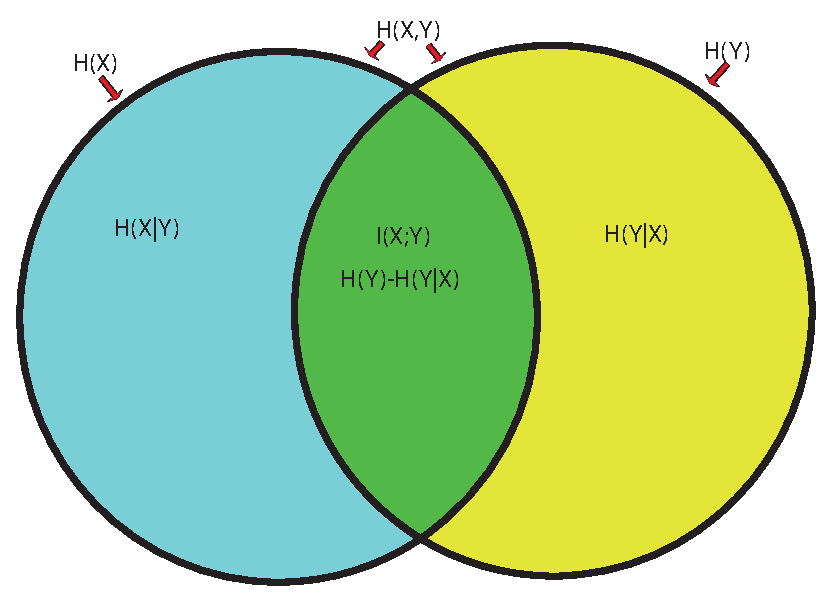
\includegraphics[scale=0.4]{Figs/venn_2_12}
				\caption{{\bf 2.12 Part e Venn Diagram}}
				\label{fig:212venn}
			\end{center}
		\end{figure}

          \end{enumerate}
          
        \item[2.15.] Markov chains: $X_{1}\rightarrow X_{2}\rightarrow \cdots \rightarrow X_{n}$, 
        		have joint probabilities of the following form: 
		\begin{eqnarray*}
			p(x_{1},x_{2},\ldots,x_{n})=p(x_{1})p(x_{2}|x_{1})\cdots p(x_{n}|x_{n-1})
		\end{eqnarray*}
		This means that for mutual information we can do some nice reduction.
		\begin{eqnarray*}
			I(X_{1};X_{2},\ldots,X_{n}) = \\
			let~~X_{3},\ldots,X_{n} = Y\\
			I(X_{1};X_{2},Y) = I(X_{1};X_{2})+I(X_{1};Y|X_{2}) \mbox{ partial application of chain rule}
		\end{eqnarray*}
		Now since this is a markov chain, and we know that $X_{1}$ and $Y$ are completely independent
		we can say that $I(X_{1};Y|X_{2})=0$ since $Y|X_{2}$ is just a subset of $Y$ which as noted
		previously is entirely independent of $X_{1}$. Thus the whole equation simplifies to $I(X_{1};X_{2})$

        \item[2.26.]
        		\begin{enumerate}[a)]
			\item $ln(x) \leq x-1$ for $0\leq x \leq \infty$
				If the second derivative of a function is positive, that means that it is concave up, or convex. If it is always greater than 0, it will never not be convex. If it could be zero on the interval, then we can't make this claim, and the converse isn't necessarily true.
				Let \(f(x)=x-1-ln\ x \) then 
				\begin{eqnarray*}
				 f'(x)= 1-\frac{1}{x}\\
				 f''(x)=\frac{1}{x^2} > 0
				 \end{eqnarray*}
				 so we can say that $f(x)$ is strictly convex and a local minimum is also a global minimum. To find the local minimum we just set $f'(x)=0$ and get $x=1$. So $f(x) \geq f(1)$ which means that $x-1-ln\ x \geq 1-1-ln\ 1 = 0$. Showing that $x-1 \geq ln\ x$ on the interval $(0,\infty)$.
			\item Justify the following steps
				Let A be the set of $x$ such that $p(x) > 0$
				\begin{eqnarray*}
				-D_e(p||q)=\sum_{x\in A} p(x) ln \frac{q(x)}{p(x)}\\
				\leq \sum_{x\in A} p(x)\left( \frac{q(x)}{p(x)}-1\right)\\
				=\sum_{x\in A} q(x) - \sum_{x\in A} p(x)\\
				\leq 0
				\end{eqnarray*}
				The first step follows from the definition of D, the second step follows from the inequality $ln\ t \leq t - 1$, the third from expanding the sum, and the last step from the fact that the $q(A) \leq 1$ and $p(A)=1$.
			\item Conditions for equality?
			We have the inequality $ln\ t \leq t-1$ from a previous problem, and showed equality iff $t=1$. Therefore we have equality if $\frac{q(x)}{p(x)}=1$ for all $x\in A$. This implies that $p(x)=q(x)$ for all $x$ and then we'll have equality in the last step as well. 
			\end{enumerate}	
          
        \item[2.32.] 
        \[P(X,Y) = \left( \begin{array}{ccc}
\frac{1}{6} & \frac{1}{12} & \frac{1}{12} \\
\frac{1}{12} & \frac{1}{6} & \frac{1}{12} \\
\frac{1}{12} & \frac{1}{12} & \frac{1}{6} \end{array} \right)\]
 where $X$ is indexed $[a,b,c]$ and $Y$ is indexed $[1,2,3]$. Let $\hat{X}(Y)$  be an estimator for $X$ based on $Y$ and let $P_e=Pr\{\hat{X}(Y)\neq X\}$
         \begin{enumerate}[a)]
        \item 
        	From inspection we see that 
        	\[\hat{X}(y)=\left\{ \begin{array}{cc}
        		1 & y=a\\
        		2 & y=b\\
        		3 & y=c \end{array}\right. \]
	and the associated $P_e$ is the sum of $P(1,b),\ P(1,c),\ P(2,a),\ P(2,c),\ P(3,a),\ P(3,b)$. Therefore $P_e=\frac{1}{2}$
        \item 
        	From Fano's inequality we know \[P_e \geq \frac{H(X|Y)-1}{log\ |\chi|}\]
        	\begin{eqnarray*}
        	H(X|Y)= H(X|Y=a)Pr\{y=a\}+H(X|Y=b)Pr\{y=b\}+H(X|Y=c)Pr\{y=c\}\\
        	=H\left(\frac{1}{2},\frac{1}{4},\frac{1}{4}\right)Pr\{y=a\}+H\left(\frac{1}{2},\frac{1}{4},\frac{1}{4}\right)Pr\{y=b\}+H\left(\frac{1}{2},\frac{1}{4},\frac{1}{4}\right)Pr\{y=c\}\\
        	=H\left(\frac{1}{2},\frac{1}{4},\frac{1}{4}\right)\left( Pr\{y=a\}+Pr\{y=b\}+Pr\{y=c\}\right)\\
        	=H\left(\frac{1}{2},\frac{1}{4},\frac{1}{4}\right)\\
        	=1.5 \mbox{ bits}
        	\end{eqnarray*}
        	Our estimator of error $P_e\geq \frac{1.5-1}{log\ 3}=0.316$ is not very close to Fano's bound in this form. Since $\hat{X}\in \chi$ we can use the stronger form of Fano's inequality 
        	\( P_e \geq \frac{H(X|Y)-1}{log(|\chi|-1)}  \) to get \( P_e \geq \frac{1.5-1}{log\ 2}=\frac{1}{2} \) which is a great bound on our actual $P_e$.
        \end{enumerate}

\end{itemize}


\end{document}

%%%%%%%%%%%%%%%%%%%%%%%%%%%%% END DOCUMENT %%%%%%%%%%%%%%%%%%%%%%%%%%%%%